\section{Estrazione dei Documenti}\label{sec:estrazione_documenti}
La fase iniziale della pipeline prevede l'estrazione del testo dai documenti normativi in formato PDF. 

Nelle prime fasi di sviluppo del progetto, l'intero documento PDF veniva passato direttamente al Large Language Model (Gemini), demandando a quest'ultimo sia il compito di estrazione del testo grezzo sia quello di strutturazione sintattica. Questo approccio presentava forti criticità, esponeva il sistema al rischio di allucinazioni ed era inefficiente nel parsing di strutture complesse. Per superare tali limitazioni, la pipeline è stata modificata separando nettamente l'estrazione del testo dalla sua successiva strutturazione.

\subsection{Open Data Loader e la Gestione dei Tagged PDF}
Per l'estrazione del testo da documenti digitali nativi è stata adottata la libreria open-source \textit{Open Data Loader}. Questo strumento consente di convertire localmente i file PDF in formati pronti per l'alimentazione degli LLM, specificamente Markdown e JSON, garantendo un'accurata ricostruzione dell'ordine di lettura e un'efficace estrazione delle tabelle e dei relativi bounding box associati agli elementi grafici. Il vantaggio di questa soluzione risiede nella sua natura puramente deterministica: a parità di input viene garantito lo stesso identico output, azzerando le variabilità tipiche dei modelli generativi in fase di pura lettura del testo.

Una delle principali problematiche riscontrate nell'estrazione da documenti legali riguarda la presenza di a capo spuri all'interno del file PDF originale, i quali, se non gestiti, introducono doppi ritorni a capo (\texttt{\textbackslash n\textbackslash n}) nel testo Markdown, frammentando artificialmente i periodi e inficiando la qualità della successiva fase di chunking. Per risolvere questa criticità, all'interno dello script di estrazione è stato configurato il parametro specifico: \texttt{use\_struct\_tree=True}.

Quando questo parametro è abilitato, la libreria verifica se il file analizzato appartiene alla categoria dei \textit{Tagged PDF}. A differenza dei PDF standard, che si limitano a definire il layout visivo e geometrico della pagina, i Tagged PDF incorporano un livello logico aggiuntivo e invisibile all'utente: il \textit{Logical Structure Tree} (Albero della Struttura Logica). Questo albero gerarchico è composto da elementi strutturali (\textit{Structural Element Nodes}) paragonabili ai tag del linguaggio HTML (quali \texttt{<H1>}, \texttt{<P>}, \texttt{<Table>}, \texttt{<L>} per le liste). Ogni porzione di testo visibile sulla pagina è mappata in modo univoco all'interno di uno di questi nodi, specificandone esplicitamente il ruolo semantico e l'esatto ordine logico di lettura, indipendentemente dalla disposizione grafica dei blocchi di testo nello spazio bidimensionale.

L'abilitazione di \texttt{use\_struct\_tree=True} permette quindi a Open Data Loader di ignorare completamente le euristiche visive o geometriche di estrazione — che spesso falliscono o introducono rumore — e di navigare direttamente lo \textit{Structure Tree} del documento. Questa tecnica consente di discriminare con precisione assoluta gli a capo puramente stilistici (dovuti ad esempio dal raggiungimento del margine della pagina) dalle effettive interruzioni di paragrafo, restituendo un testo continuo, pulito e semanticamente fedele all'originale.

% INIZIO YAPPING SUPREMO 
Nel contesto specifico di questo lavoro di tesi, focalizzato sui documenti normativi e sugli atti amministrativi della Pubblica Amministrazione Locale, l'approccio basato sui Tagged PDF si è rivelato straordinariamente efficace per ragioni sia pratiche che legali. Le istituzioni pubbliche sono infatti vincolate da stringenti obblighi normativi in materia di accessibilità digitale. Tali norme impongono che ogni documento pubblicato sui portali istituzionali sia pienamente fruibile anche da utenti con disabilità visive o motorie attraverso l'uso di tecnologie assistive, come gli screen reader.

La conformità a questi standard garantisce che il \textit{Logical Structure Tree} del PDF non solo sia presente, ma risulti strutturato accuratamente: i testi seguono una gerarchia rigida, le tabelle possiedono intestazioni chiare per righe e colonne, e l'ordine logico di lettura è validato direttamente alla fonte. Di conseguenza, quello che per l'ente pubblico rappresenta un adempimento di legge obbligatorio, si traduce in una vera e propria ``ancora di salvezza''.
% FINE YAPPING SUPREMO


\subsection{Docling e l'Integrazione dei Motori OCR}
L'approccio standard basato su Open Data Loader mostra evidenti limiti in presenza di documenti non strutturati, privi di testo selezionabile o derivanti da scansioni visive, in quanto la libreria non integra nativamente un modulo OCR. Per sopperire a questa mancanza e gestire layout documentali complessi, è stata introdotta nel sistema la libreria \textit{Docling}, un motore avanzato di parsing e analisi del layout specializzato nell'estrazione di metadati, tabelle e testo da formati complessi, integrato nella pipeline come supporto a Open Data Loader.

L'introduzione dell'OCR ha sollevato complessità non trascurabili relative alla gestione delle risorse hardware all'interno dell'architettura a container. Il container Docker deputato all'estrazione operava infatti con un vincolo stringente di memoria RAM pari a un massimo di 4 GB, per questioni di risorse hardware. Durante i primi test, l'invio massivo di interi documenti scansionati causava la saturazione istantanea della memoria, provocando l'intervento del modulo del kernel Linux (\textit{Out-Of-Memory Killer}) che terminava forzatamente il container.

Per superare il problema del consumo di RAM e prevenire i crash di sistema, è stata implementata una strategia basata sull'elaborazione pagina-per-pagina e si è proceduto a un'attività di comparazione su tre diversi motori OCR supportati da Docling:
\begin{enumerate}
    \item \textbf{EasyOCR:} Configurato di default all'interno di Docling, adotta modelli basati su Deep Learning altamente accurati ma estremamente esigenti in termini computazionali. Anche isolando l'elaborazione sulla singola pagina, il consumo di RAM superava costantemente la soglia critica dei 4 GB, rendendone impossibile l'utilizzo nell'ambiente di produzione containerizzato.
    \item \textbf{Tesseract OCR:} Si è dimostrato estremamente leggero e pienamente compatibile con i limiti di memoria imposti, scongiurando qualsiasi crash del container. Tuttavia, nel contesto specifico del linguaggio legale italiano, il motore non è stato in grado di interpretare correttamente il layout, fallendo l'estrazione del testo e restituendo all'interno del file Markdown unicamente i link di riferimento alle immagini scansionate.
    \item \textbf{RapidOCR:} Questo specifico modulo è stato infine selezionato per l'estrazione del testo dalle scansioni visive. RapidOCR si è rivelato il compromesso ingegneristico ideale, offrendo un perfetto bilanciamento tra l'accuratezza del riconoscimento del testo italiano e il consumo di RAM del container, che si è mantenuto costantemente sotto la soglia di guardia. A fronte di un tempo di computazione non trascurabile — quantificabile in circa 18-20 secondi per singola pagina scansionata — questo motore assicura la totale stabilità infrastrutturale dell'intera pipeline.
\end{enumerate}

\subsection{Progettazione del Custom Triage Processor}
Il processore di triage nativo di Open Data Loader prevede un flusso standard in cui ogni pagina viene analizzata e smistata: le pagine semplici vengono processate tramite il processo di Open Data Loader (una JVM), mentre le pagine complesse vengono delegate al backend basato su Docling. 

Tuttavia, l'applicazione con l'uso del parametro \texttt{use\_struct\_tree=True} introduce un bug logico nel triage di default: i documenti non espressamente \textit{tagged} vengono forzati all'interno del processo standard di Open Data Loader, non venendo mai instradati verso il backend di Docling, escludendo così l'analisi per pagine troppo complesse oppure l'attivazione dell'OCR dove necessario.
Per risolvere questa problematica è stato progettato e implementato un \textbf{Custom Triage Processor}. Il componente agisce secondo la seguente logica di controllo:

\begin{itemize}
    \item \textbf{Fase 1: Verifica preliminare della struttura.} 
    Non appena il file PDF viene acquisito, il sistema ne analizza i metadati per verificare se è codificato come \textit{Tagged PDF}. In caso affermativo, l'intero documento viene elaborato direttamente da Open Data Loader sfruttando l'albero strutturale nativo. Questo approccio garantisce la massima velocità di esecuzione e una pulizia ottimale del testo estratto.
    
    \item \textbf{Fase 2: Frazionamento del documento e stima della complessità.} 
    Se il documento risulta privo di struttura (\textit{Non-Tagged}), viene diviso in singole pagine indipendenti. Questa separazione è fondamentale per prevenire sovraccarichi di memoria RAM durante le elaborazioni successive. Per ciascuna pagina, il sistema calcola poi la densità dei caratteri testuali per valutarne il grado di complessità.
    
    \item \textbf{Fase 3: Triage ed elaborazione mirata della pagina.} 
    Sulla base dell'analisi precedente, ogni singola pagina subisce un processo di smistamento intelligente per essere indirizzata allo strumento di estrazione più adeguato:
    \begin{itemize}
        \item Se la pagina presenta un layout lineare e un'elevata densità di testo nativo, viene classificata come \textit{Semplice} e affidata al processo di Open Data Loader.
        \item Se la pagina contiene elementi geometrici articolati o tabelle annidate, ma il testo rimane comunque selezionabile, viene classificata come \textit{Complessa} e processata tramite \textit{Docling Standard} (senza abilitare l'OCR).
        \item Se la pagina è priva di testo nativo (es. una fotocopia), viene classificata come \textit{Scansione} e inviata al container specializzato di \textit{Docling}, dove interviene il motore \textit{RapidOCR} per il riconoscimento ottico dei caratteri.
    \end{itemize}
\end{itemize}

L'intero processo appena descritto è schematizzato nella Figura \ref{fig:triage-processor}.

\begin{figure}[H]
    \centering
    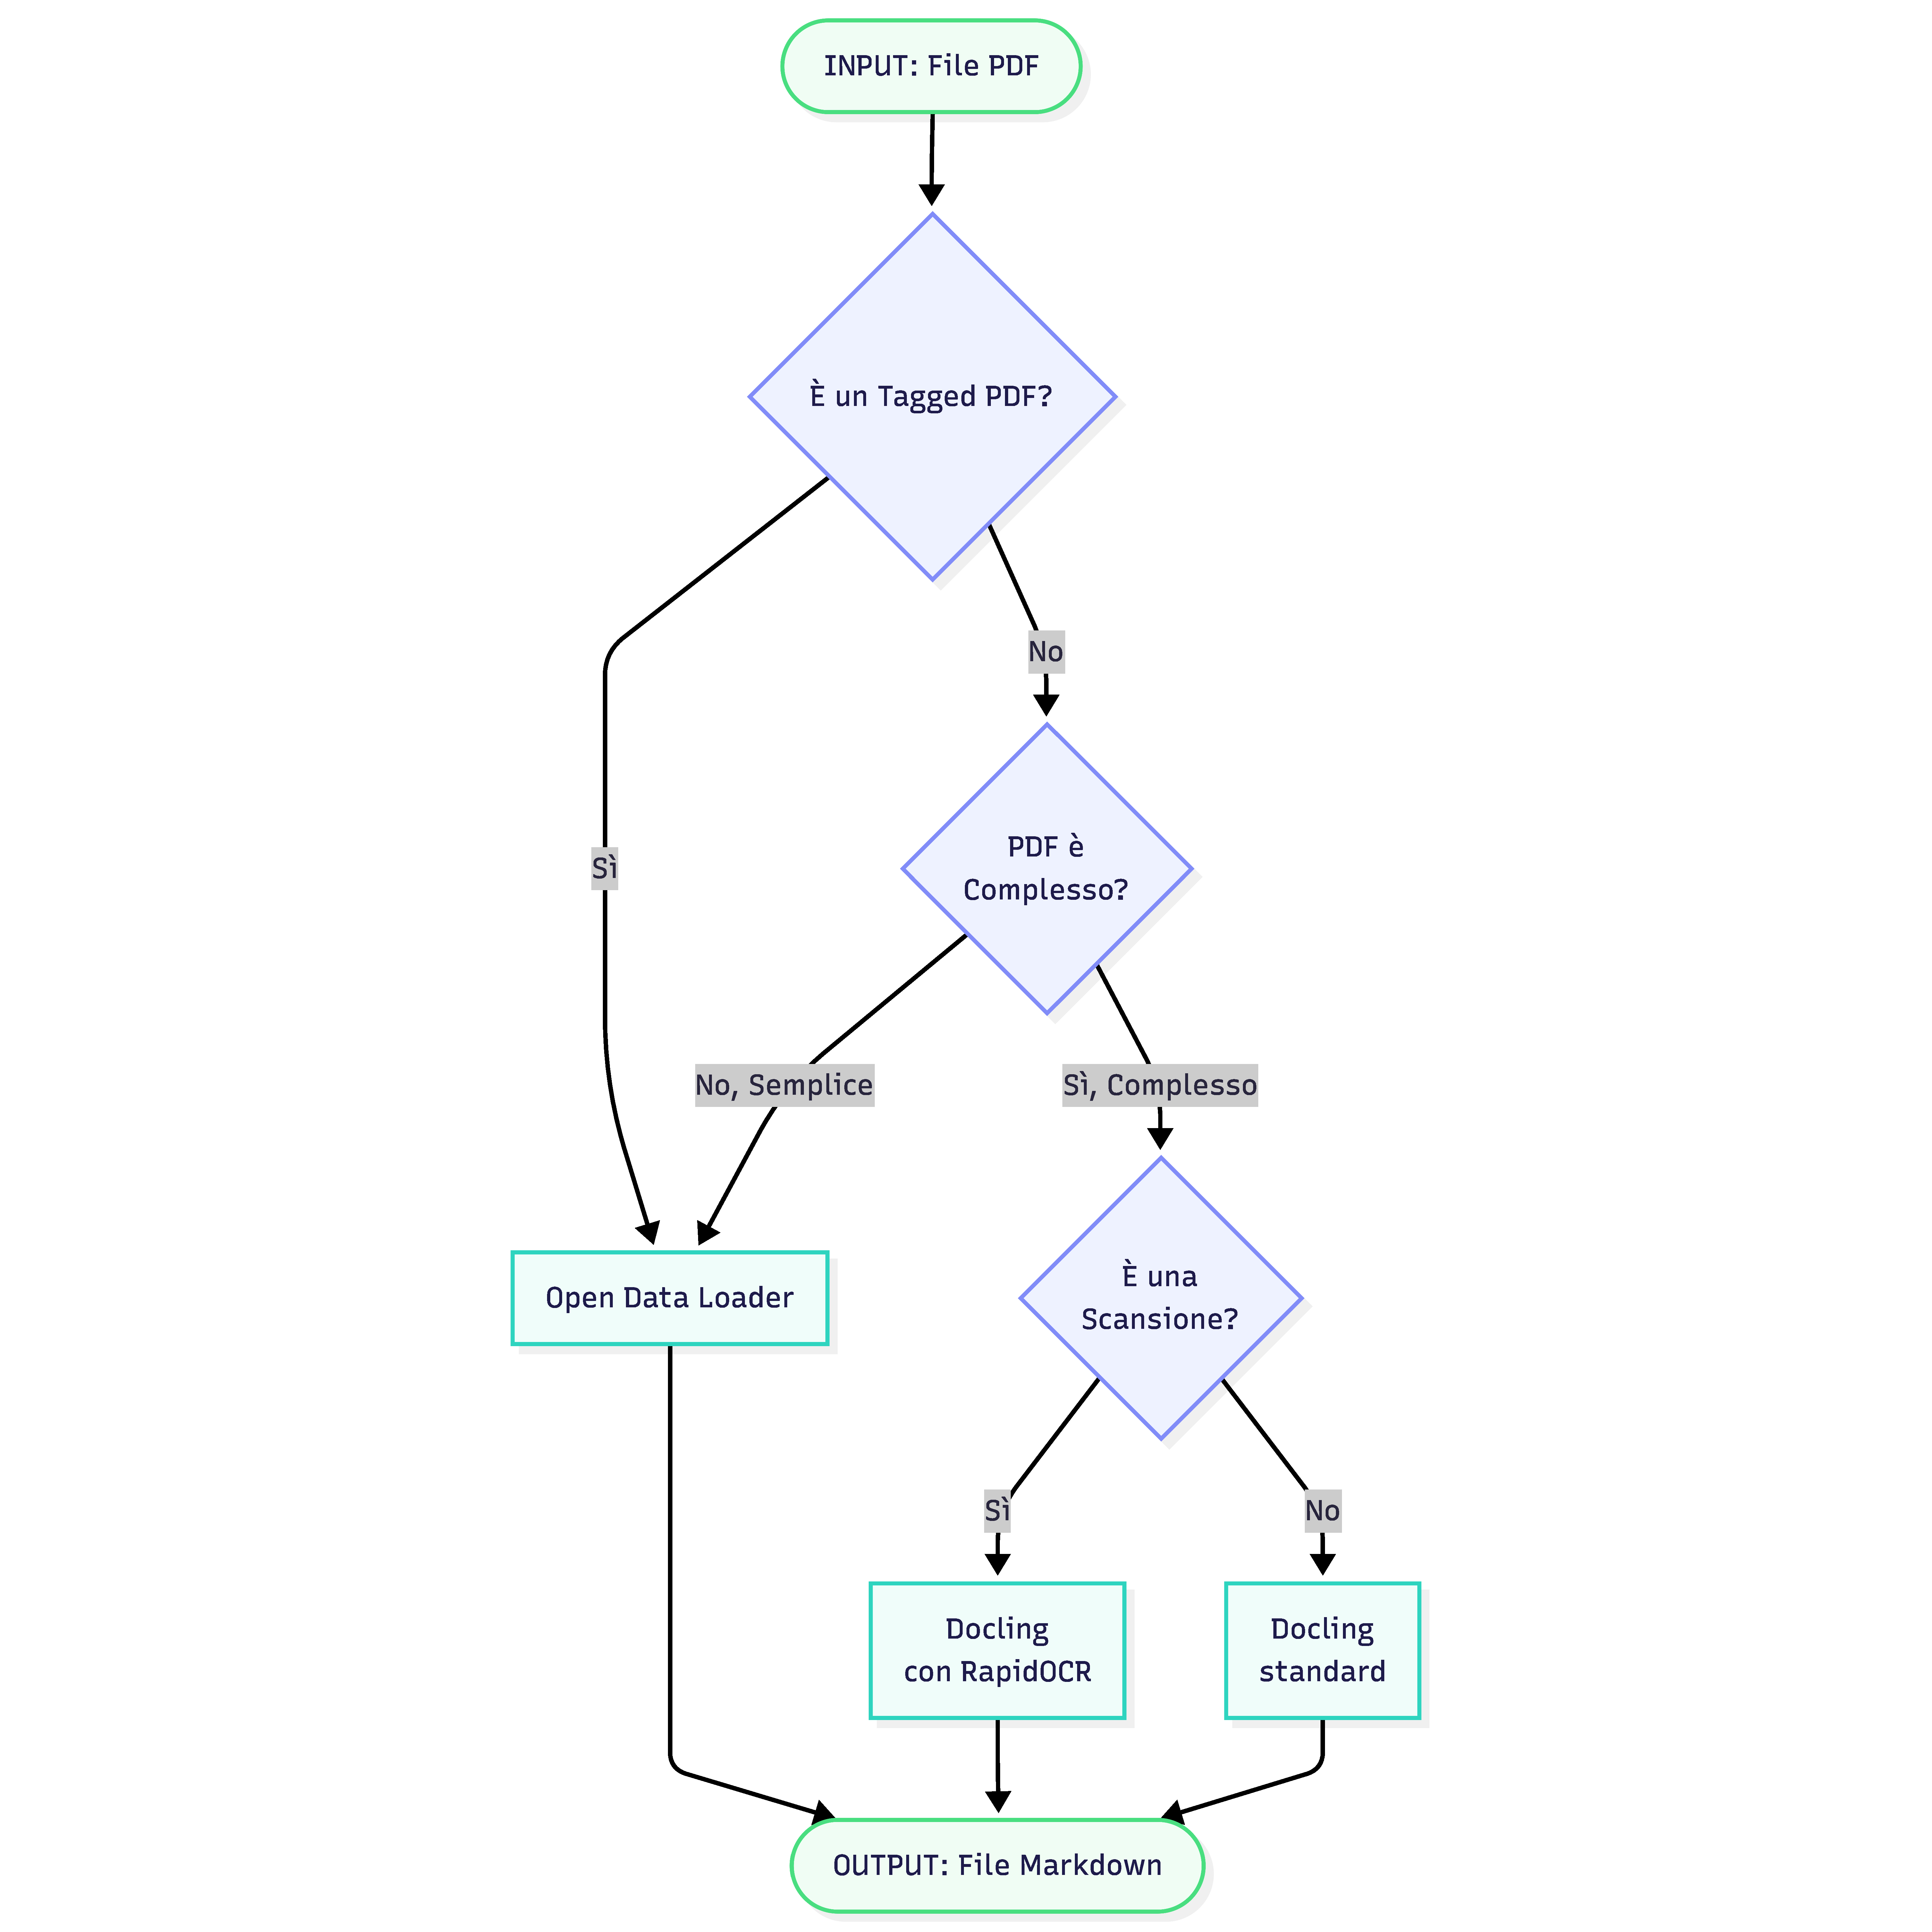
\includegraphics[width=1\textwidth]{_images/triage-processor.pdf}
    \caption{Flowchart del Custom Triage Processor}
    \label{fig:triage-processor}
\end{figure}
\newpage